\documentclass{article}
\usepackage[utf8]{inputenc}

\title{PS6}
\author{Alex Skipper }
\date{February 2018}

\usepackage{natbib}
\usepackage{graphicx}
\usepackage{float}

\begin{document}
\maketitle


\section{Visualization 1}

The first visualization comes from Kaggle, a link is in the rscript, and contains information about Terrorist Incidents around the globe from 1970 to 2016. \\

Cleaning:\\
The data was ordered yearly with multiple variables, so I created a subset of the original data, pulling data regarding to North America called R1. From R1, I pulled the years and countries into separate vectors, then proceeded to merge them into a data frame. Additionally I renamed the columns to more useful terms.  From there I used the table command in R to show the frequency and after that I converted it into a data frame.
\\
The data is showing where most of these incidents are happening in North America, which helps show the changes in frequency and location of terrorist incidents in North America. Is helpful for understanding the data by showing a visualization measure of frequency, which is easier to understand than looking at a spreadsheet. 
\\
\begin{figure}[H]
\centering
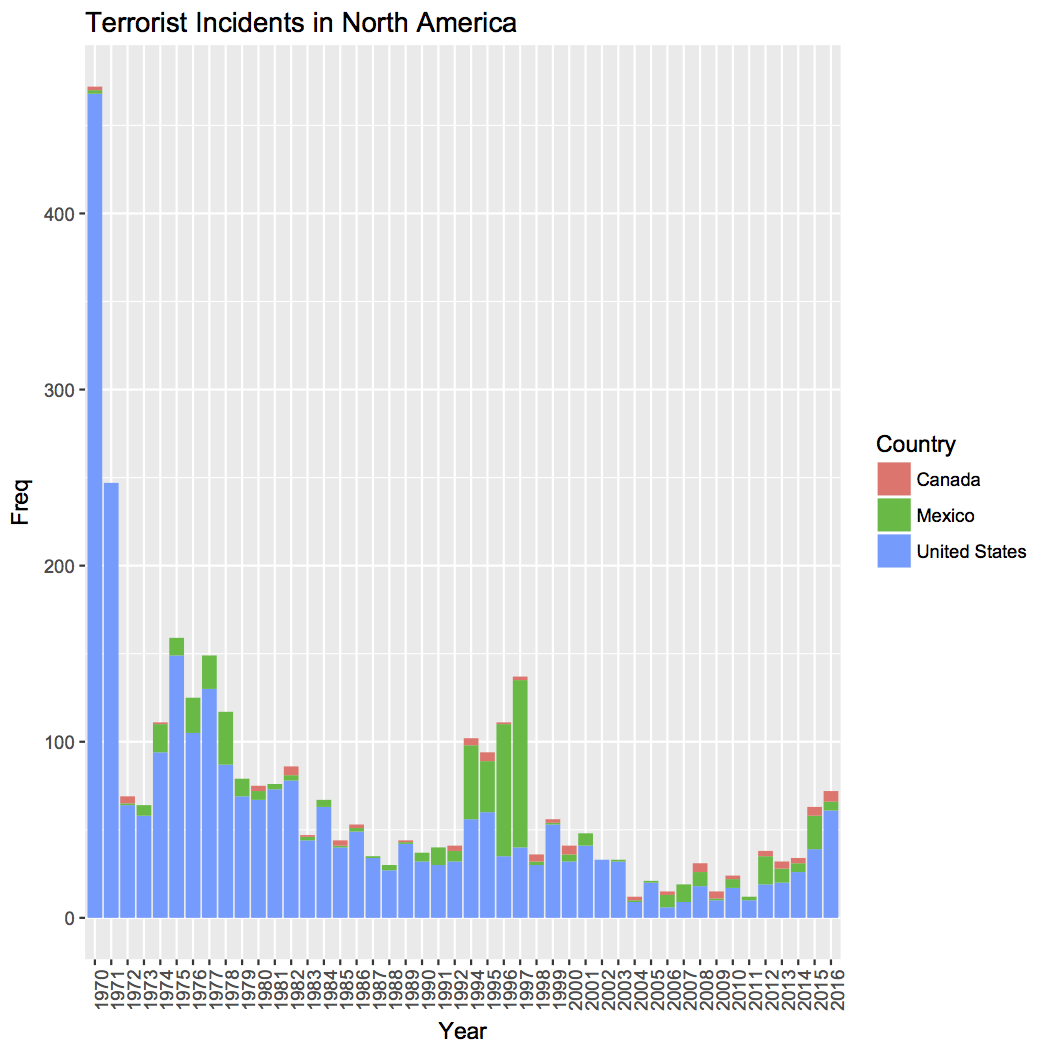
\includegraphics[scale=.8]{Visual_1_PS6.png}
\end{figure}\\
\newpage

\section{Visualization 2}


The second visualization comes from stock market data pulled from Yahoo, and contains stock yearly returns and daily closing prices for Microsoft and Apple.\\
\\
Cleaning visual 1:\\
First, I had to pull the data from Yahoo, R had a package that does it for you (In the Rscript). I wanted yearly returns, so running the command yearlyreturns, I created a variable for both Microsoft and Apple and merged them together. I also had to rename the column titles.\\
\\
Side Note: Had a hard time using ggplot on this visualization, so I didnt use it for this one. But I cleaned and transformed the data to try to get it to work partially. I took the yearlyreturns variables and merged them. After the merge, I took the merge and made it a data frame. However, the id column was the years, so I transformed the data frame to shift the column over and become a variable, which seems ggplot likes. 
\\
The data is showing the annual returns of these two tech giants from the time they went public to whenever you pull the data in R. It also helps show the volatility  in the tech market.  Helpful for understanding the data set by showing if there any correlation between these two stocks from first observing a visualization.But it needs to be confirmed that these two might be correlated.\\
\\
\begin{figure}[H]
\centering
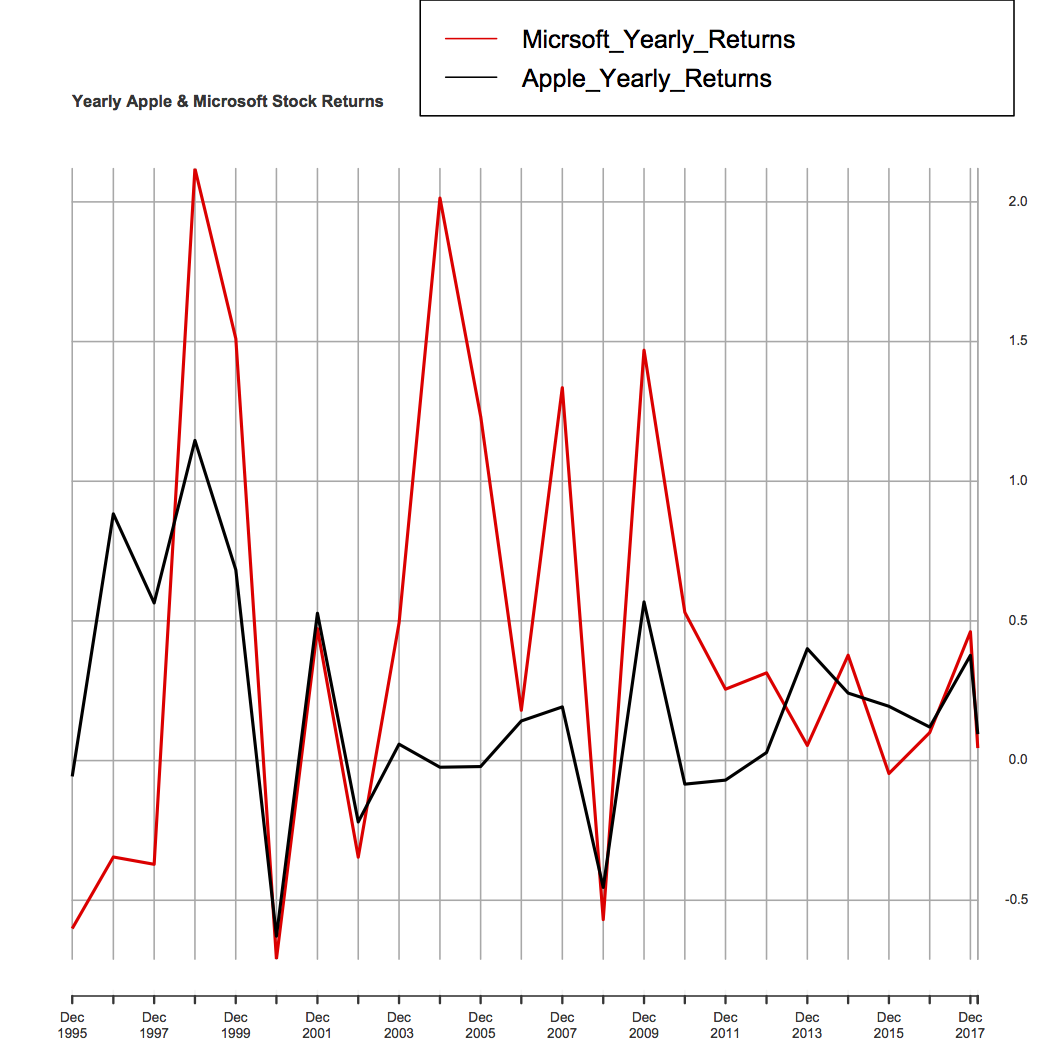
\includegraphics[scale=.8]{Visual_2_1_PS6.png}
\end{figure}
\newpage
\\
Cleaning visual 2:Finding the correlation between AAPL and MSFT
I had to create data frame with the pulled variables relating to closing price and merge the two/ to get the daily return percentages, I created another data frame and transformed it with the diff command to calculate the lag difference by one day and to set it up in a matrix so it does the diff command to all columns. \\
\\
\begin{figure}[H]
    \centering
    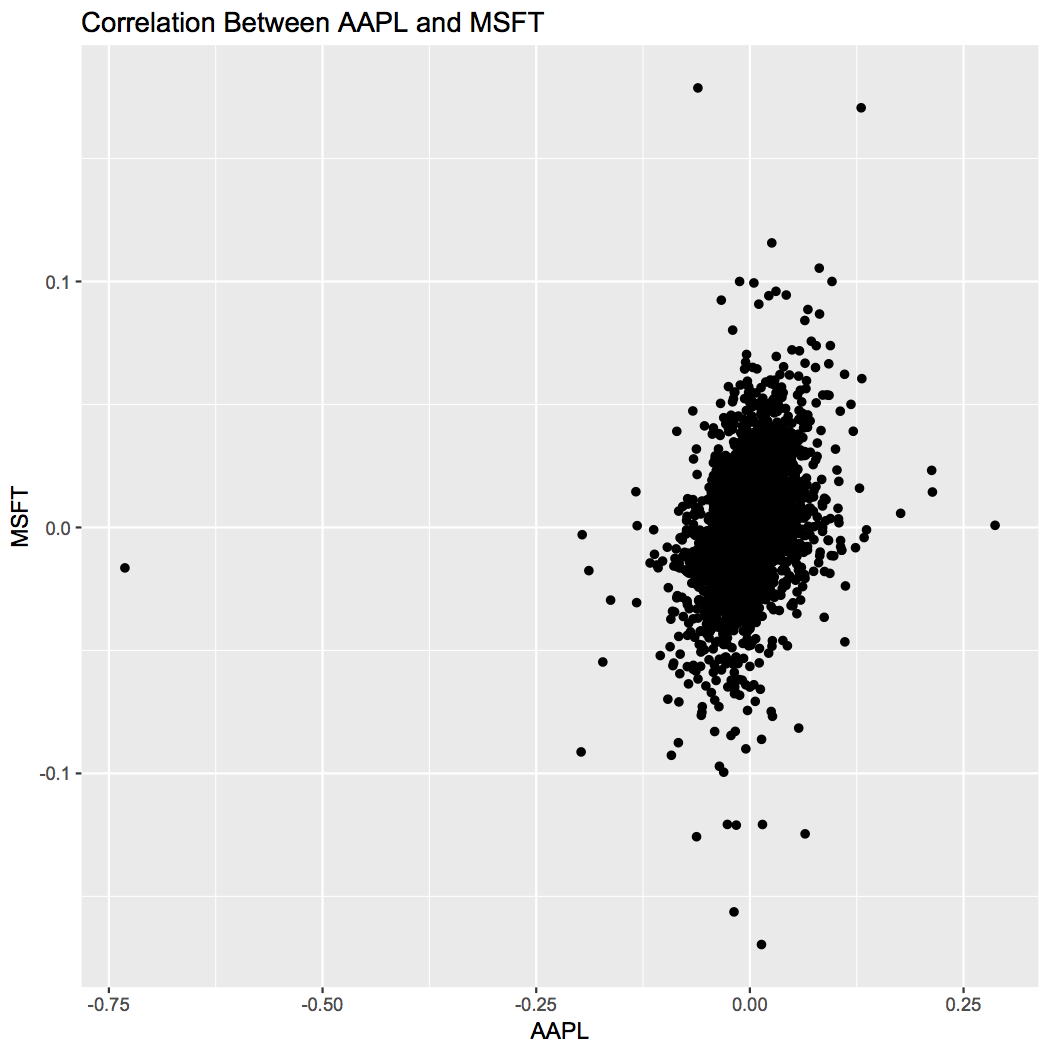
\includegraphics[scale=.8]{Visual_2_2_PS6.png}
\end{figure}
\newpage

The data is showing the correlation between the two stocks indicating that these two stocks are positive correlated. Helpful for understanding  the data set by showing the correlation between these two stocks and whether or not they're good investments. (Done on an extremely small scale). A more information to back up the ideas about visual 1.

\section{Visualization 3}

Same as the first visualization, regarding the data and source, but shows the total sum that terrorist incidents happened each year throughout the globe.\\
\\
Cleaning:\\
There wasn't as much cleaning to do with this one, but I had to pull the year and region text from the data to create a data frame. From there I used the table command to get the frequency of incidents that happened each year. While also changing the column names to make it easier to graph on ggplot. \\
\\
The data is communicating that there has been in a steady increase in terrorist related incidents since 2003 and has exponentially skyrocketed. Helpful for understating the data by showing the direction or frequency these incidents are happening. The data shows that there is a growing problem that needs to be addressed by governments in order to combat this issue. (As we have seen in the news throughout the years, it is a lot easier said then done.) Government work may of resulted in a decrease after 2014, but more information is needed to truly understand if Government played a role. 
\\
\begin{figure}[H]
\centering
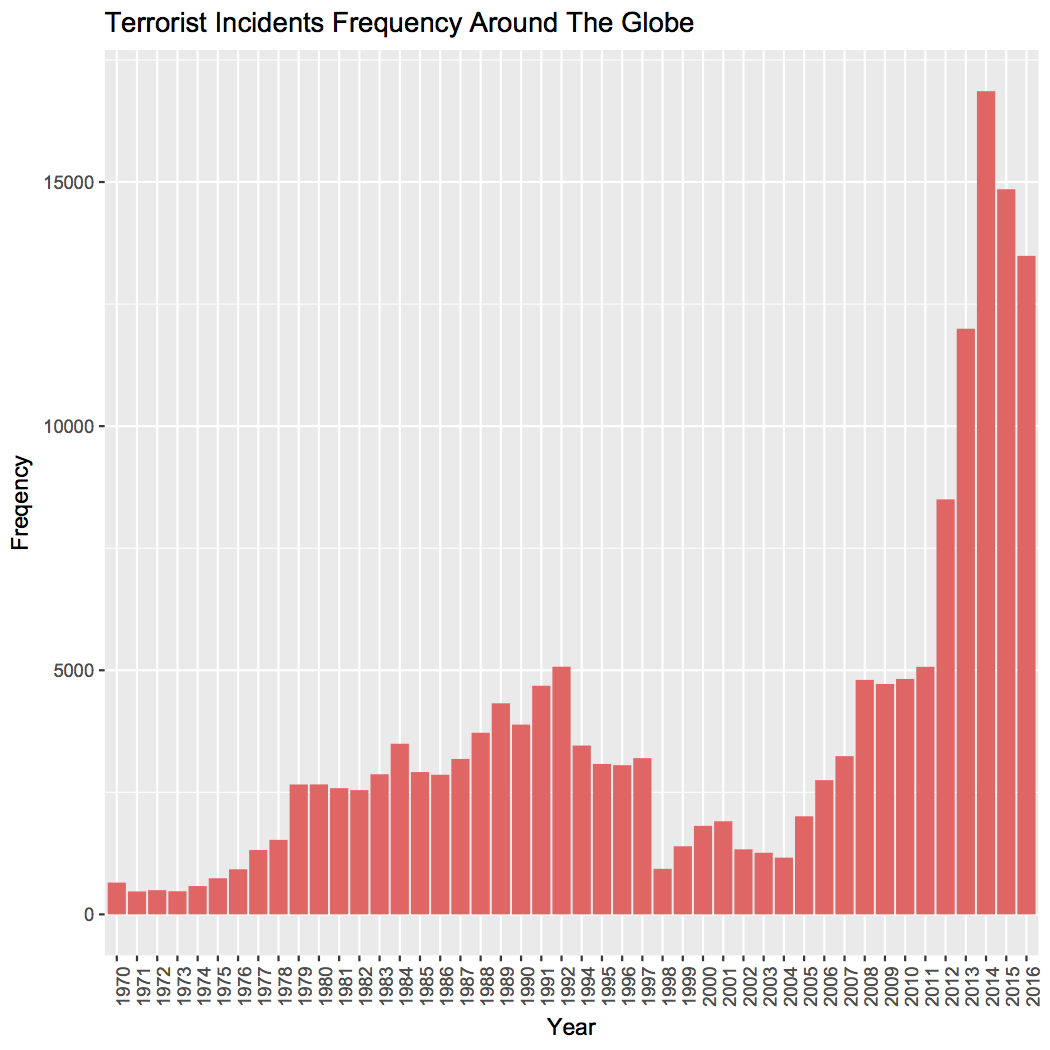
\includegraphics[scale=.8]{Visual_3_PS6.png}
\end{figure}

\end{document}